\section{OpAmps AC}

Der Operationsverstärker ist in allgemeiner Näherung ein Tiefpass-Filter n-ter Ordnung mit linearer Verstärkung.

 \begin{tabular}{|p{0.15\linewidth}|p{0.28\linewidth}|p{0.445\linewidth}|}
 	\hline
 	Frequenzgang allgemein
 		& \large{$A(s) = \frac{A_{0}}{(1+\frac{s}{\omega_{p_1}})(1+\frac{s}{\omega_{p_2}})\dots}$}
 		& $A_{0}=$ Lineare Verstärkung \newline $\omega_{p_i}=$ Polkreisfrequenzen \\
 	\hline
 \end{tabular}
 
\subsection{Open-Loop/Closed-Loop Verhalten}

\begin{tabular}{|p{0.45\linewidth}|p{0.45\linewidth}|}
	\hline
	\textbf{Open-Loop}
		& \textbf{Closed-Loop}\\
	\hline
	\multicolumn{2}{|c|}{\textbf{Blockschemas}}\\
	\hline
    \vspace{-7mm}
	\begin{center}
	 	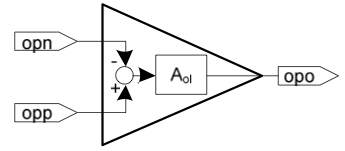
\includegraphics[height=2cm, valign=t]{./pictures/opAmpOL.png}
	\end{center}
		& \vspace{-7mm}
          \begin{center}
			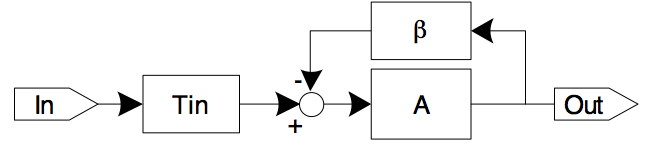
\includegraphics[height=2cm, valign=t]{./pictures/opAmpCL.png}
		  \end{center}\\
	\hline
	\multicolumn{2}{|c|}{\textbf{Frequenzgänge}}\\
	\hline
	\large{$A_{ol}(s)=\frac{A_{ol_0}}{(1+\frac{s}{\omega_{p_{ol_1}}})(1+\frac{s}{\omega_{p_{ol_2}}})\dots}$}
	& $\begin{aligned}
        A_{cl}(s) &= \frac{A_{cl_0}}{(1+\frac{s}{\omega_{p_{cl_1}}})(1+\frac{s}{\omega_{p_{cl_2}}})\dots} = \frac{T_{in}(s)\cdot A_{ol}(s)}{1+\beta(s)\cdot A_{ol}(s)}\\
		\beta(s) &= \frac{V_{opn}}{V_{out}}\;\text{oder}\;\frac{V_{opp}}{V_{out}}\\
		T_{in}(s) &= \frac{V_{opn}}{V_{in}}\;\text{oder}\;\frac{V_{opp}}{V_{in}}\\
        V_{out} &= A_{cl}(s)\cdot V_{in} = \frac{T_{in}(s)\cdot A_{ol}(s)}{1 + \underbrace{A_{ol}(s)\cdot \beta(s)}_{T_s(s):Loop-Gain}} \cdot V_{in}
	   \end{aligned}$\\
	\hline
\end{tabular}
\\ \\
\begin{tabular}{m{0.45\linewidth}m{0.45\linewidth}}
	Durch das Schliessen des Loops wird die Bandbreite vergrössert, das gain-bandwidth-product(GBP) bleibt jedoch konstant. Die Verstärkung wird jedoch um $T_{s0}(s)$ (Linearer Loop Gain) reduziert. Der Phasengang wird durch das Verschieben des ersten Poles auch verändert, wie folgende Grafik zeigt.
	& \begin{center}
        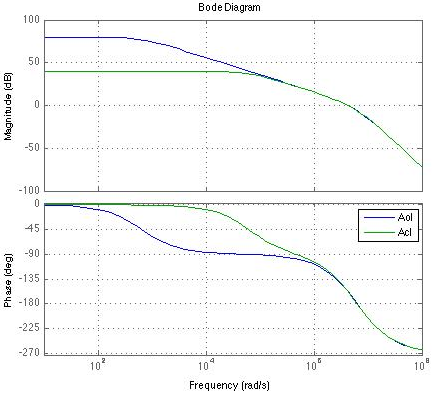
\includegraphics[width=6.7cm, valign=t]{./pictures/AolAcl.png}
    \end{center}
\end{tabular}
\vspace{-7mm}
\subsection{Stabilität des Systems}
\begin{tabular}{m{0.45\linewidth}m{0.45\linewidth}}
    Um die Stabilität des OpAmps zu betrachten, wird der Loop geöffnet. Damit das System stabil ist, darf das       
    Fehlersignal sich selbst nicht verstärken. Damit dies der Fall ist muss die Phase $>-180^\circ$ sein bei einem Loop Gain von $1$, da das Vergleichsglied die Phase noch um $180^\circ$ dreht. 
    
    Ein Mass für die Stabilität ist die 
    Phasenmarge (Phase Margin) und die Verstärkungsmarge (Gain Margin). Optimal ist ein Phase Margin von $60^{\circ}$.
    
    Die UTF ist dann stabil, wenn sie nie $\infty$ wird d.h der Nenner darf nie 0 werden.
    & \begin{center}
        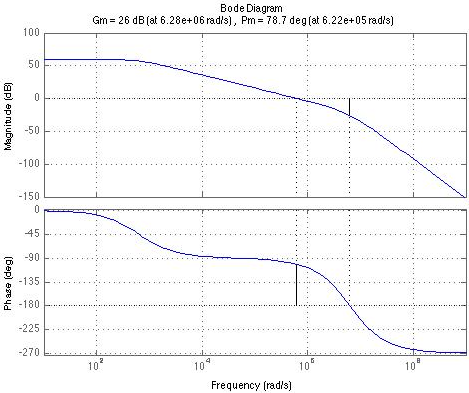
\includegraphics[width=5cm, valign=t]{./pictures/margins.png}
    \end{center}
\end{tabular}

%  ---------------------------------------------------------------------------------------------------- 
